\section{Introduction}
\showtoc

\subsection{Motivation}
\begin{frame}
  \frametitle{Goal}
  goal
\end{frame}

%\subsection{History}
\begin{frame}[t]
  \only<1> {
    {\Large \bf Biomechanics}
    \begin{itemize}
    \item
      D.~A. Winter, {\em Biomechanics and Motor Control of Human Movement}, 2nd ed., New York: Wiley-Interscience, 1990.\\
    \item
      J. Perry and J. Burnfield, Gait Analysis: Normal and Pathological Function, 2nd ed., Thorofare: Slack Inc., 2010.\\
    \end{itemize}
  }
  \only<2,3> {
    \textcolor{gray}{\Large \bf Biomechanics}\\[1mm]
  }

  \only<2> {
    {\Large \bf Reduction-Based Control}
    \begin{itemize}
    \item
      A.~D. Ames et al., {\em On the Geometric Reduction of Controlled Three-Dimensional Bipedal Robotic Walkers}, in 3rd Workshop on Lagrangian and Hamiltonian Methods for Nonlinear Control (LHMNL'06), Nagoya, Japan, Jul. 2006.\\
    \item
      R.~W. Sinnet et al., {\em 3D Bipedal Walking with Knees and Feet: A Hybrid Geometric Approach}, in 48th IEEE Conference on Decision and Control, Shanghai, P. R. China, Dec. 2009.
    \item
      R~.W. Sinnet and A.~D. Ames, {\em Bio-Inspired Feedback Control of Three-Dimensional Humanlike Bipedal Robots}, in Journal of Robotics and Mechatronics, special issue on {\em Focused Areas and Future Trends in Bio-Inspired Robots}, Aug. 2012.

    \end{itemize}
  }
  \only<1,3> {
    \textcolor{gray}{\Large \bf Reduction-Based Control}\\[1mm]
  }

  \only<3> {
    {\Large \bf Human-Inspired Control}
    \begin{itemize}
    \item
      A.~D. Ames, {\em First Steps Toward Automatically Generating Bipedal Robotic Walking from Human Data}, in 8th International Workshop on Robotic Motion and Control, Gron{\'o}w, Poland, Jun. 2011.
    \item
      R.~W. Sinnet et al., {\em A Human-Inspired Hybrid Control Approach to Bipedal Robotic Walking}, in 18th IFAC World Congress (IFAC 2011), Milan, Italy, Sep. 2011.
    \item
      R.~W. Sinnet et al., {\em A Human-Inspired Framework for Bipedal Robotic Walking Design}, International Journal of Biomechatronics and Biomedical Robotics, Jan. 2014.
    \end{itemize}
  }
  \only<1,2> {
    \textcolor{gray}{\Large \bf Human-Inspired Control}
  }

\end{frame}

\begin{frame}
  \frametitle{History}
  \begin{columns}

    \begin{column}{.24\textwidth}
      \textcolor{blue}{Passive Walking:}
      \begin{figure}
        \centering
        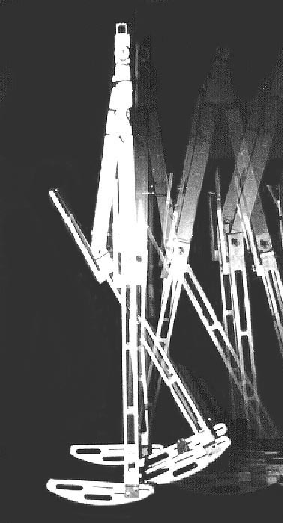
\includegraphics[height=4.5cm]{bipeds_ruina}
      \end{figure}
    \end{column}

    \begin{column}{.24\textwidth}
      \textcolor{blue}{Passivity-Based Control:}
      \begin{figure}
        \centering
        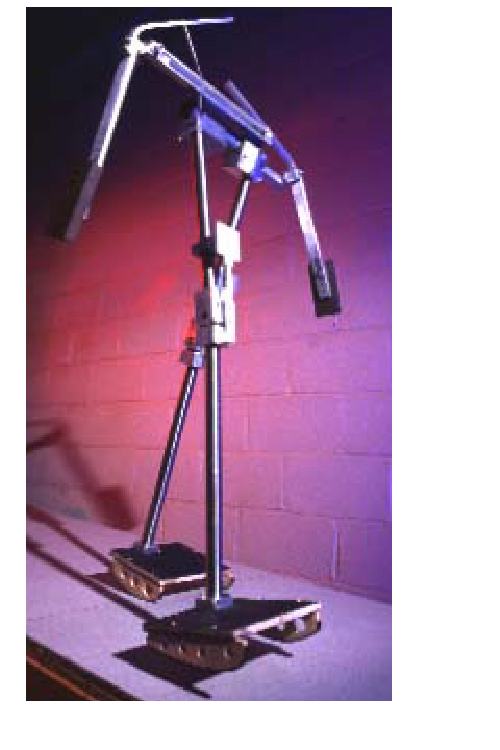
\includegraphics[height=4.5cm]{bipeds_collins}
      \end{figure}
    \end{column}

    \begin{column}{.24\textwidth}
      \textcolor{blue}{Hybrid Zero Dynamics:}
      \begin{figure}
        \centering
        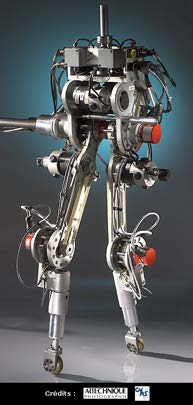
\includegraphics[height=4.5cm]{figures/bipeds_grizzle}
      \end{figure}
    \end{column}

    \begin{column}{.24\textwidth}
      \textcolor{blue}{Human-Inspired Control:}
      \begin{figure}
        \centering
        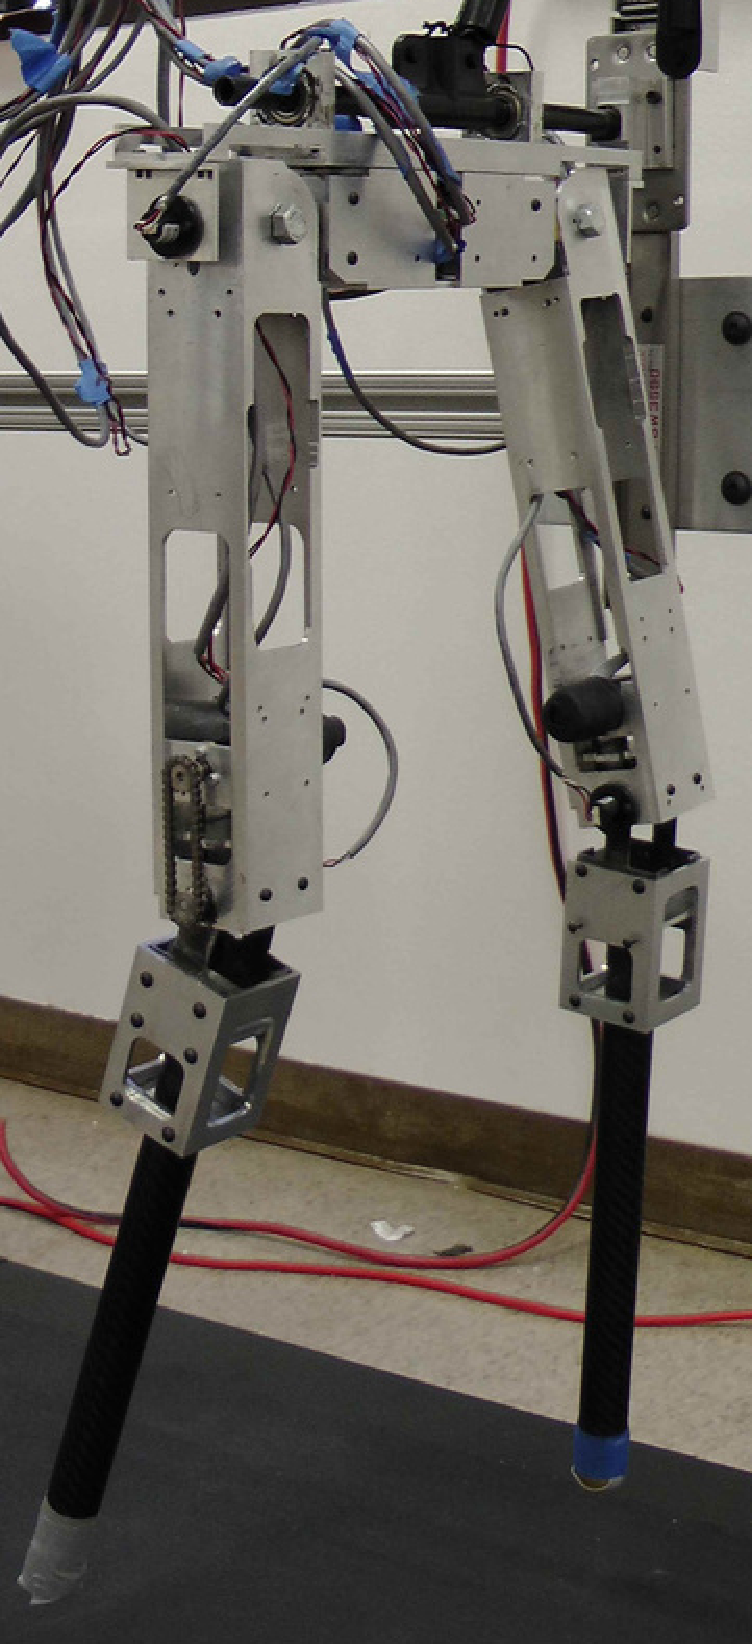
\includegraphics[height=4.5cm]{figures/bipeds_ames}
      \end{figure}
    \end{column}

  \end{columns}
\end{frame}
